\documentclass{article}
\usepackage{tikz}
\usepackage{amsmath, amsfonts}
\pagestyle{empty}

\begin{document}
\begin{figure}
  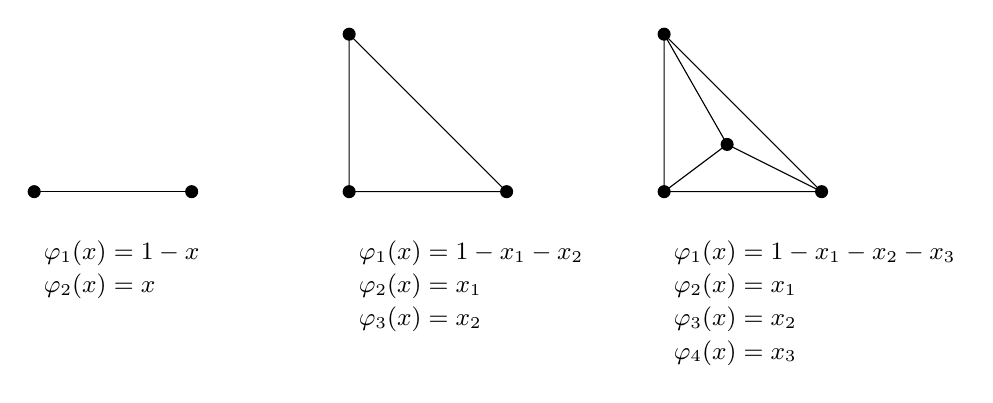
\begin{tikzpicture}
    % 1D interval
    \draw (0,0) -- (2,0);
    \draw[black,fill=black] (0,0) circle (.5ex);
    \draw[black,fill=black] (2,0) circle (.5ex);
    \node[below right, align=left] at (0,-0.5)
        {\small $\varphi_1(x) = 1 - x$ \\
         \small $\varphi_2(x) = x$};
   
    % 2D triangle
    \draw (4,0) -- (6,0) -- (4,2) -- (4,0);
    \draw[black,fill=black] (4,0) circle (.5ex);
    \draw[black,fill=black] (6,0) circle (.5ex);
    \draw[black,fill=black] (4,2) circle (.5ex);
    \node[below right, align=left] at (4,-0.5)
        {\small $\varphi_1(x) = 1 - x_1 - x_2$ \\
         \small $\varphi_2(x) = x_1$ \\
        \small $\varphi_3(x) = x_2$};

    % 3D tetrahedron
    \draw (8,0) -- (10,0) -- (8,2) -- (8,0);
    \draw (8,0) -- (8.8, 0.6);
    \draw (10,0) -- (8.8, 0.6);
    \draw (8,2) -- (8.8, 0.6);
    \draw[black,fill=black] (8,0) circle (.5ex);
    \draw[black,fill=black] (10,0) circle (.5ex);
    \draw[black,fill=black] (8,2) circle (.5ex);
    \draw[black,fill=black] (8.8,0.6) circle (.5ex);
    \node[below right, align=left] at (8,-0.5)
        {\small $\varphi_1(x) = 1 - x_1 - x_2 - x_3$ \\
         \small $\varphi_2(x) = x_1$ \\
         \small $\varphi_3(x) = x_2$ \\
         \small $\varphi_4(x) = x_3$};
  \end{tikzpicture}
  \caption{Lagrange $\mathbb{P}_{1}$ shape functions in 1D, 2D and 3D.}
\end{figure}
\end{document}